\section{Coarse-grained simulations}

During the discussion of the nanopiston's operation cycle it was hypothesised
that entropic interactions play an important role in its functioning. Studying these
phenomena is experimentally rather difficult, since all results are inferred based upon
the measured current traces and known interactions between the different elements of the
system. To obtain a more in-depth understanding of these interactions, computer
simulations are needed to proved the necessary insights.

In view of these challenges, a coarse-grained model of the DNA nanopiston was devised by
Bayoumi et al. The model is used to perform molecular dynamics simulations of  the
conformational fluctuations of the rotaxane at zero bias. Performing the simulations was
done by using the Large-scale Atomic/Molecular Massively Parallel Simulator (LAMMPS) and
its implementation of a Langevin intergrator.[.]

The coarse-grained model is composed of four types of interacting pseudo
atoms, all taking into account excluded volume interactions via repulsive Lennard-Jones
potentials. First of all, the Clya nanopore is represented by three vertically stacked
open cylinders, with diameters 6 nm, 5.5 nm and 2.9 nm from the cis- to the trans-side.
To take into account the electrostatic DNA-nanopore interactionsthe, the cylinder radii
are appropriately adjusted from the pore's geometry reported in.[.]
These electrostatic interactions predominately arise from excess negative charge in the
constriction of ClyA, resulting in a reduced size of the trans-cylinder. Note that the
pore is excluded from the Langevin integration, resulting in a static pore model.

A semiflexible bead-and-spring model is used to simulate the rotaxane. Each spherical
bead represents one ssDNA nucleotide or five dsDNA base pairs, respectively having a
diameter of $1\ nm$ and  $2.2\ nm$. The bond connecting each consecutive pair of beads is
represented by a harmonic spring. Determining the bond stiffness is done by means of the
equipartition theorem, from which we find
  \begin{equation}
    k_{bond} = \frac{3 k_b T }{ \langle a \rangle},
  \end{equation}
here $\langle a \rangle$ is the equilibrium bond length taken to be $0.68\ nm$ or $1.7\
nm$ for ssDNA and dsDNA respectively. In this model the bending rigidity of the DNA
polymer is taken into account. This effect is modelled as previous seen in the discrete
worm like chain, where the angle between consecutive bond vectors is assigned a harmonic
potential. Using Equation .., the bending rigidity is determined by
  \begin{equation}
    \kappa_{bend} = \frac{l_{p} \kappa_b T}{\langle a \rangle},
  \end{equation}
  where $l_p$ is the persistence length of the ssDNA ($2.2\ nm$) and dsDNA ($45\ nm$)
strands. The difference in persistence length results in the relatively large flexibility
of ssDNA strands.

The last components of the coarse-grained model are the neutravidin protein stoppers,
which capture the rotaxane inside of the nanopore. During experiments it was observed
that the neutravidin proteins entered the lumen of ClyA. Using this information the size
of the spherical stoppers was fitted to reproduce this behaviour using simulations. The
found diameter is $7\ nm$. The lipid bilayer in which the pore is embedded also interacts
with these proteins, this is simulated by a reflective boundary at the lower entrance of
the nanopore.

Using the above described model, simulations where the conformational fl


% 3) conclusie -> inderdaad werd gevonden dat de entropy
% belangrijk was, discuss limits.
%    crude approximation -> not that physically accurate results and no hybridisation

% The crucial role of entropy has also been demonstrated in another class of rotaxanes,
% composed of dsDNA and ssDNA of varying lengths
% Discuss limits of the model. Limited accuracy of the CG model since it does not caputre
% the full structure of DNA accurately. For example the double helix structure is note
% captured. Another consequence is that the DNA hybridisation can not be simulated using
% this model, since both ssDNA nucleotides and dsDNA basepairs are represented by simple
% beads. To further analyse and understand the operation cycle of the nanopiston a more
% accurate CG model is needed.

\begin{figure}[ht]
  \begin{centering}
  \adjustbox{minipage=1.3em,valign=t}{\subcaption{}\label{sfig:testa}}%
  \begin{subfigure}[t]{\dimexpr.4\linewidth-1.3em\relax}
  \centering
  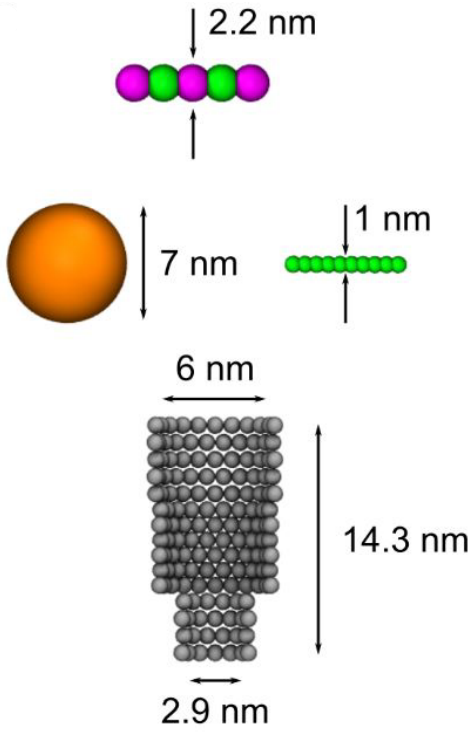
\includegraphics[width=0.9\linewidth,valign=t]{Figures/Stefanos1.png}
  \end{subfigure}%
  \adjustbox{minipage=1.3em,valign=t}{\subcaption{}\label{sfig:testb}}%
  \begin{subfigure}[t]{\dimexpr.5\linewidth-1.3em\relax}
  \centering
  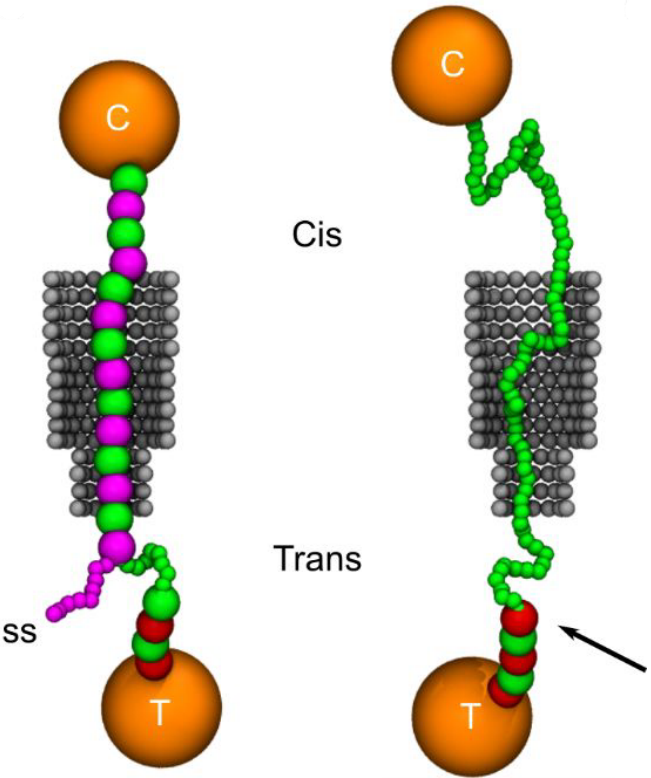
\includegraphics[width=0.9\linewidth,valign=t]{Figures/Stefanos2.png}
  \end{subfigure}
  \caption{This is a figure}
  \label{fig:test}
  \end{centering}
\end{figure}

